\newpage
\appendix

\section{Mouvement horizontal}
\begin{figure}[H]
  \centering
	\begin{subfigure}{.45\linewidth}
		\centering
		\includegraphics[width=\textwidth]{figures/horizontal-pos.pdf}
		\caption{Position en $x$}
		\label{fig:x-bound-pos}
	\end{subfigure}
	\begin{subfigure}{.45\linewidth}
		\centering
		\includegraphics[width=\textwidth]{figures/horizontal-v.pdf}
		\caption{Vitesse en $x$}
		\label{fig:x-bound-v}
	\end{subfigure}

	\begin{subfigure}{.5\linewidth}
		\centering
		\includegraphics[width=\textwidth]{figures/horizontal-alpha.pdf}
		\caption{Accélération en $x$}
		\label{fig:x-bound-alpha}
	\end{subfigure}

	\caption{Attributs du point $A$ lorsque contraint à un mouvement horizontal}
	\label{fig:x-bound}
\end{figure}

\begin{figure}[H]
  \centering
\begin{subfigure}{.26\linewidth}
		\centering
		\includegraphics[width=\textwidth]{figures/x-bound-fig-before.pdf}
		\caption{lorsque $\theta=0$}
		\label{fig:x-bound-before}
	\end{subfigure}
	\hspace{1cm}
	\begin{subfigure}{.2\linewidth}
		\centering
		\includegraphics[width=\textwidth]{figures/x-bound-fig-after.pdf}
		\caption{lorsque $\theta=\frac{\pi}{3}$}
		\label{fig:x-bound-after}
	\end{subfigure}
		\caption{Positionnement du bras contraint à un mouvement en $x$ selon $\theta$}
	\label{fig:x-bound-figs}
\end{figure}

\section{Mouvement vertical}

\begin{figure}[H]
  \centering
	\begin{subfigure}{.48\linewidth}
		\centering
		\includegraphics[width=\textwidth]{figures/vertical-pos.pdf}
		\caption{Position en $y$}
		\label{fig:vertical-pos}
	\end{subfigure}
	\begin{subfigure}{.48\linewidth}
		\centering
		\includegraphics[width=\textwidth]{figures/vertical-v.pdf}
		\caption{Vitesse en $y$}
		\label{fig:vertical-v}
	\end{subfigure}

	\caption{Attributs du point $A$ lorsque contraint à un mouvement horizontal}
	\label{fig:vertical-plots}
\end{figure}

\begin{figure}[H]
  \centering
	\begin{subfigure}{.36\linewidth}
		\centering
		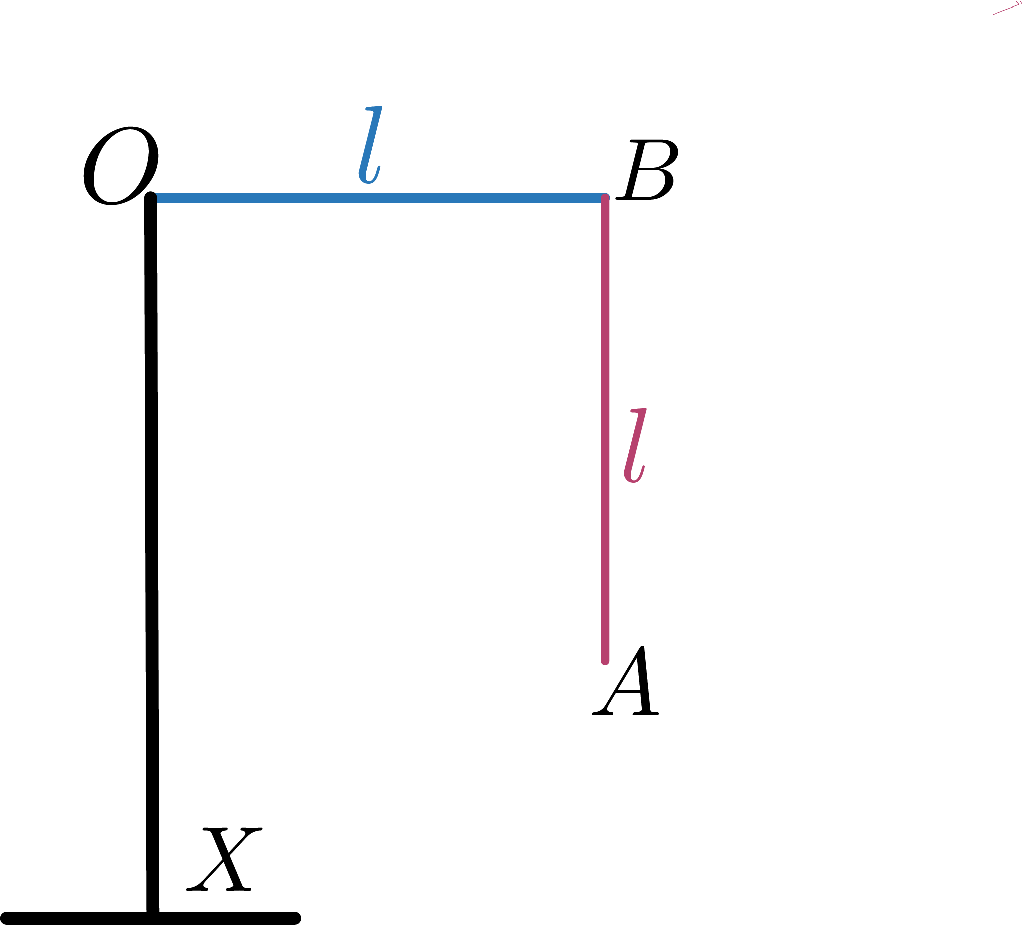
\includegraphics[width=\textwidth]{figures/vert-before.pdf}
		\caption{lorsque $\theta=0$}
		\label{fig:vert-before}
	\end{subfigure}
	\hspace{1cm}
	\begin{subfigure}{.3\linewidth}
		\centering
		\includegraphics[width=\textwidth]{figures/vert-after.pdf}
		\caption{lorsque $\theta=\frac{\pi}{3}$}
		\label{fig:vert-after}
	\end{subfigure}
		\caption{Positionnement du bras contraint à un mouvement en $y$ selon $\theta$}
	\label{fig:vert-figs}
\end{figure}

\section{Simulations statiques et dynamiques}

\begin{figure}[H]
  \centering
  \includegraphics[width=0.7\textwidth]{figures/static-torque.pdf}
  \caption{Couple résultant $M_{B_z}$ en fonction de l'angle $\varphi$ (cas statique)}
  \label{fig:static-torque}
\end{figure}

\todo{Dynamique: Plot $C_b$ selon $\varphi$}
